\section{Systems with changing mass}
\paragraph{Second Law of Newton}
$$\vec{F} = \frac{d}{dt}\left( m \vec{v} \right) = \frac{dm}{dt}\vec{v} + m\frac{d\vec{v}}{dt} = \dot{m}\vec{v}+m\vec{a}$$
$$\vec{F} = \frac{d\vec{p}}{dt}$$
\begin{itemize}
	\item $\vec{a}$ doesn't have to be in same direction as $\vec{v}$. 
	\item You should be accurate in calculating $\dot{m}\vec{v}$ since $\vec{v}$ depends on frame of reference 
\end{itemize}

\paragraph{Example} Plank of area $\vec{S}$ moves with velocity $\vec{v}$ and gathers dust which density is $\rho$. At $t=0$ mass of plank is $M_0$ and velocity is $\vec{v}_0$. What is acceleration of plank and dependency of velocity of time.


\begin{center}
	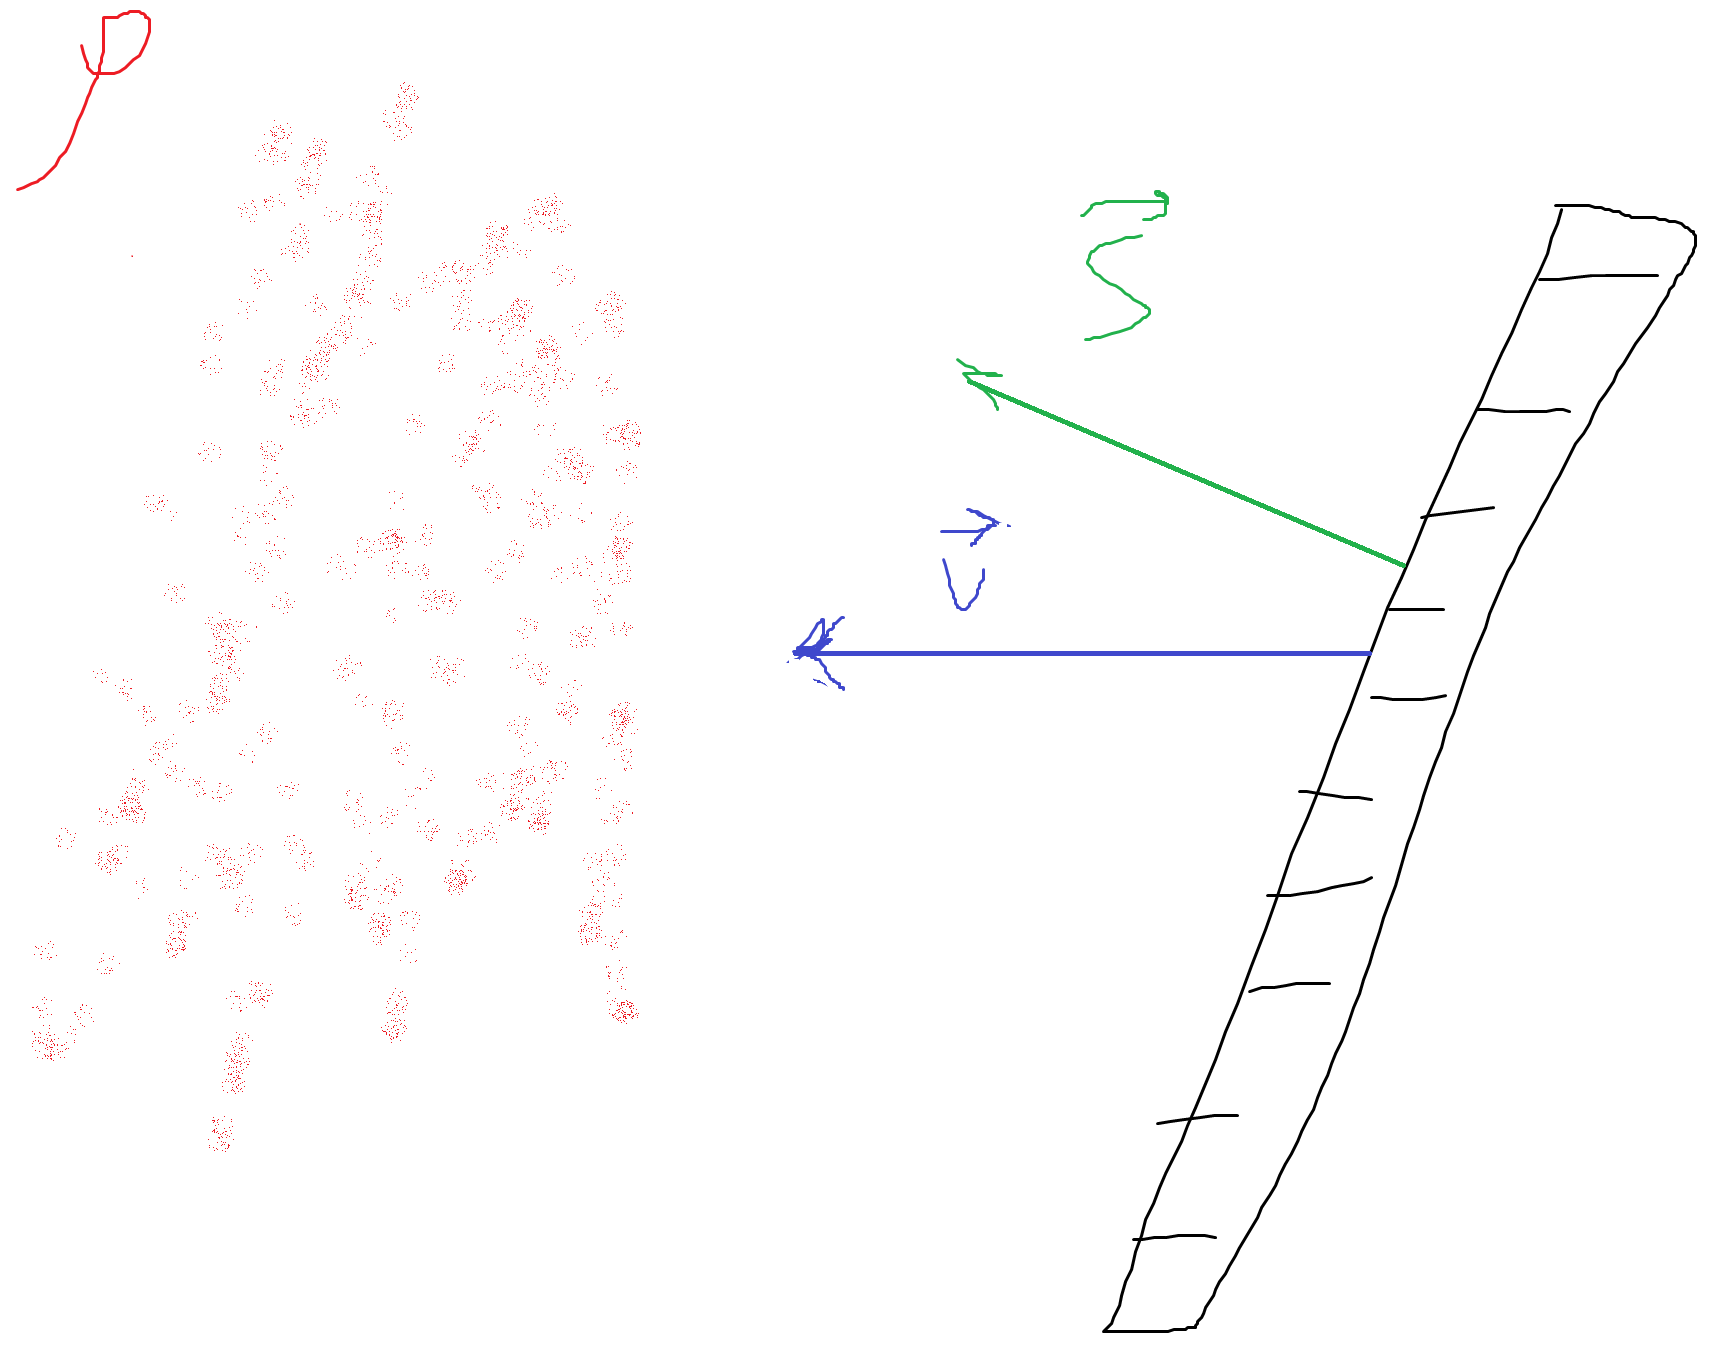
\includegraphics[width=\linewidth]{./lect13/pic1.png}
\end{center}

Volume of parallelepiped is $\Delta V = \left( \Delta t v \right) S \cos \theta = \vec{v} \cdot \vec{S} \Delta t$

Mass gathered in time $\Delta t$ is $\Delta m = \Delta V \rho$. And speed of mass change is

$$\dot{m} = \frac{dm}{dt} = \frac{\Delta m}{\Delta t}= \frac{\vec{v} \cdot \vec{S} \Delta t}{\Delta t} \rho= \vec{v}\vec{S}\rho = vS\rho \cos \theta$$

Since $\rho, S, \cos \theta$ are constant, denote $k = S \rho \cos \theta$ meaning $\dot{m} = kv$.


There are three ways to solve the problem:
\begin{enumerate}
	\item System of plank and cloud  (reference point of cloud). There is no external forces, the momentum is conserved. 
	$$0  = F_{ext} = \frac{d}{dt} \left( m_{total} \vec{v}_{total} \right)$$
	$$0 = \dot{m}v + m\dot{v} + \dot{m}_{cloud} \underbrace{v_{cloud}}_{0} + m_{cloud}\underbrace{\dot{v}_{cloud}}_{0}$$
	$$\frac{\dot{v}}{v}= - \frac{\dot{m}}{m}$$
	$$\frac{1}{v} \frac{dv}{dt} = - \frac{1}{m} \frac{dm}{dt}$$
	$$\frac{dv}{v}=\frac{dm}{m}$$
	Now solve integral with initial conditions
	
	$$\int_{v_0}^{v} \frac{d v^\prime}{v^\prime} = - \int_{m_0}^{m} \frac{d m^\prime}{m^\prime} $$
	$$\left[ \ln v^\prime \right]^v_{v_0} = - \left[ \ln m^\prime \right]^m_{m_0}   $$
	$$\ln \frac{v}{v_0} = \ln \frac{m_0}{m} $$
	$$ \frac{v}{v_0} = \frac{m_0}{m} $$
	$$ m = \frac{v_0m_0}{v} $$
	
	From $\frac{\dot{v}}{v}= - \frac{\dot{m}}{m}$ we acquire:
	
	$$\dot{v} = \frac{dv}{dt} = -\frac{\dot{m}}{m}v \stackrel{\dot{m} = kv}{=} -\frac{kv}{\frac{m_0v_0}{v}}v  = -\frac{k}{m_0v_0}v^3$$
	
	We need to solve differential equation $\frac{dv}{dt} = -\frac{k}{m_0v_0}v^3$:
	$$\frac{dv}{v^3} = - \frac{k}{m_0v_0} dt$$.
	Integral is:
	
	$$ \int_{v_0}^{v(t)} \frac{dv}{v^3} = -\int_{0}^{t} \frac{k}{m_0v_0} dt^\prime $$
	
	$$\left[ -\frac{1}{2} v^{-2}\right]^{v(t)}_{v_0} = -\frac{k}{m_0v_0}t$$
	$$-\frac{1}{2} \frac{1}{v^2} + \frac{1}{2}\frac{1}{v_0^2} = -\frac{k}{m_0v_0}t$$
	
	With solution:
	
	$$v = \left( \frac{2k}{m_0v_0}t + \frac{1}{v_0^2} \right)^{-\frac{1}{2}}$$
	\item Force on plank changes velocity of cloud in frame of reference  of cloud in $t=0$. There is a change in impulse of cloud.
	
	$$\underbrace{f_c}_{\parbox{2cm}{\centering \scriptsize force of plank on cloud}} = \frac{dp_{cloud}}{dt} = \frac{p_{end}-p_{begin}}{\Delta t}$$
	
	Initial velocity of cloud is 0 and terminal velocity is $v$ (frame of reference  of cloud in $t=0$): $p_{begin} = \Delta m \cdot 0$ and  $p_{begin} = \Delta m \cdot v$.
	
	So $f_c= \frac{\Delta m v}{\Delta t} = \dot{m}v$ and $F_{p} = -f_c  = - \dot{m}v$.
	
	In a very short time change in mass is negligible (the force which cloud exerts on plank is exerted only on particles which were already on plank after previous moment). So we can use second law of Newton:
	$$m \dot{v} = F_{p} = -\dot{m}v \Rightarrow \dot{v} = -\frac{\dot{m}}{m}v = -\frac{k}{m} v^2$$
	\item We choose frame of reference in which at time $t$ velocity of plank $v(t) =  0$.
	
	Just like in 1, total impulse is conserved.
	
	$$0 = \frac{d}{dt}p_{total} = \frac{d}{dt} \left( m v^\prime + m_{cloud} v^\prime_{cloud} \right)$$
	
	where $v^\prime$ is a velocity in our frame of reference.
	
	$$0 = \dot{m} v^\prime + m\underbrace{\dot{v}^\prime}_{0} + \dot{m}_{cloud} v^\prime_{cloud} + m_{cloud}\underbrace{ \dot{v}^\prime_{cloud}}_{0}$$
	
	Velocity of cloud doesn't changes (the velocity of frame of reference is constant) and also velocity of plank doesn't changes according to definition. But $v^\prime_{cloud} \neq 0$, and $v^\prime_{cloud}  = -v$. Since the reference point isn't accelerating, $\dot{v}^\prime = \dot{v}$. By substituting $\dot{m}_{cloud} = -\dot{m}$  acquire:
	
	$$m\dot{v} + \dot{m}v = 0$$
\end{enumerate}	
	
\section{Angular momentum}

Angular momentum is a conserved value due to rotation symmetry.

Angular momentum of single particle relative to origin (in inertial frame of reference) $$\vec{J} = \vec{r} \times \vec{p} = \vec{r} \times \left( m \vec{v} \right)$$


\begin{center}
	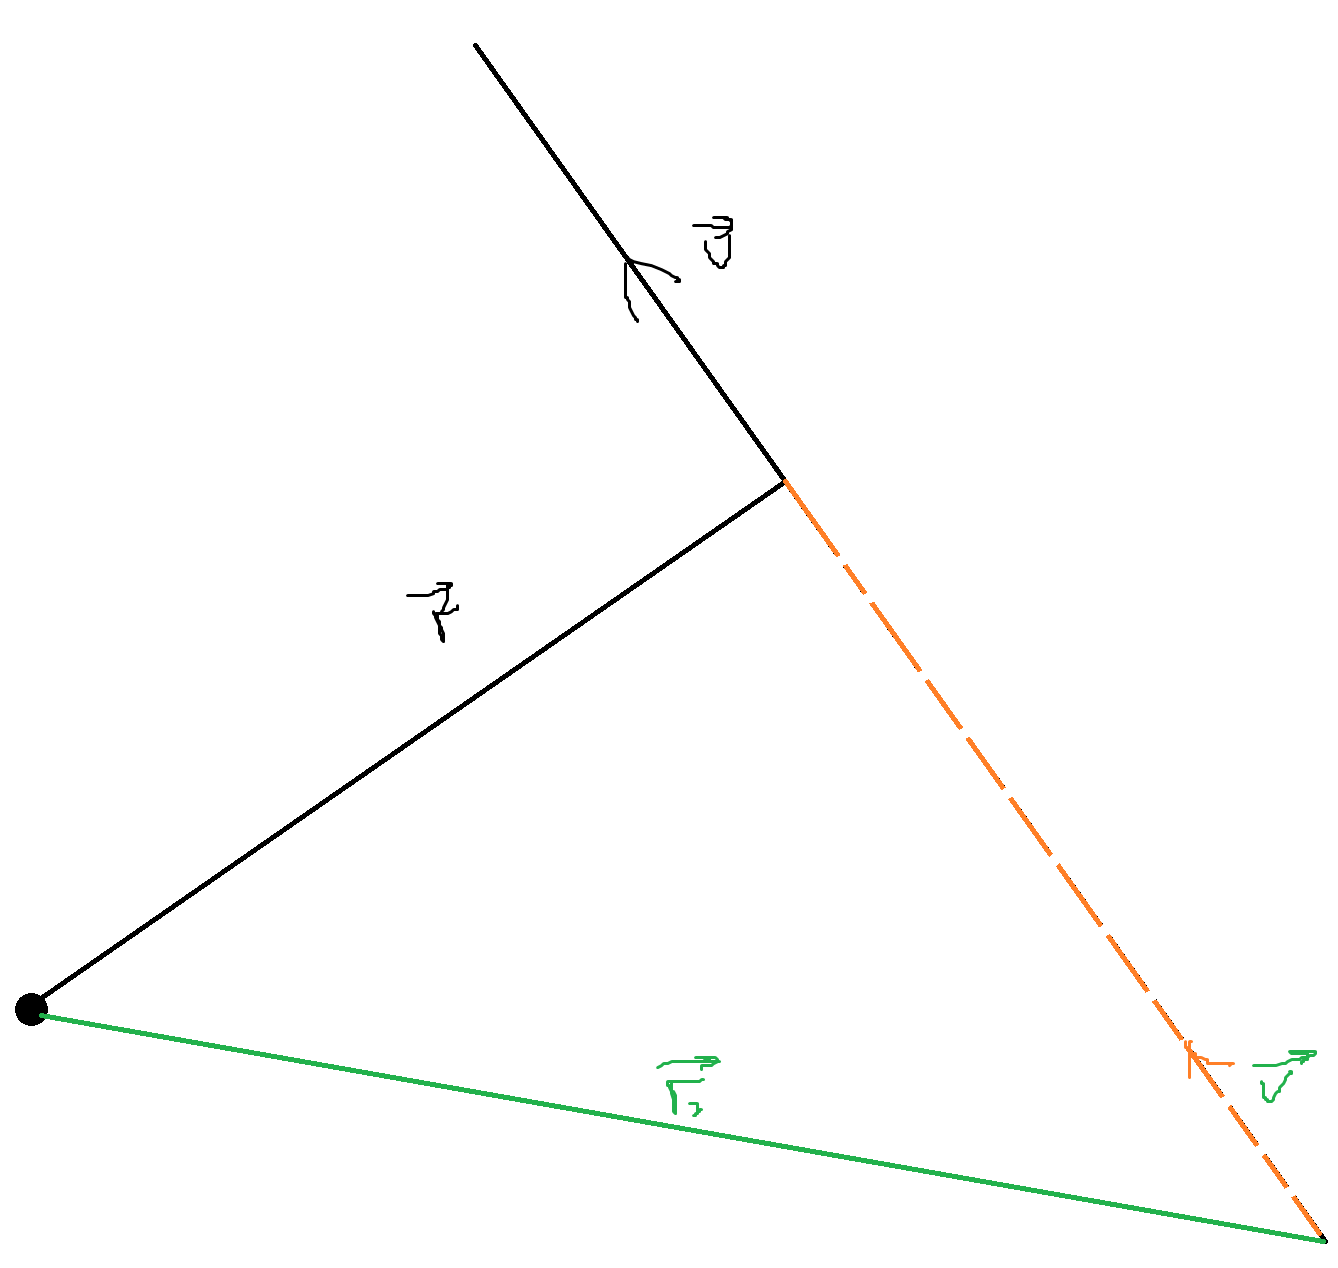
\includegraphics[width=0.2\linewidth]{./lect13/pic2.png}
\end{center}


$$\vec{J}=\vec{J}_2$$.